\section{Question 4}

{\bfseries Try to slowly increase or decrease the (edge) threshold. Comment
why the number of detected keypoints decreases when the threshold is decreased.
Is this the expected behavior according to the way the threshold is defined?}

The edge threshold is used to filter out extrema of the difference of Gaussians that lie on an edge, i.e. that have a small curvature. Keypoints on edges can be moved along the edges with minor differences in their features and are thus not well suited to be selected. Figure \ref{fig:inc_edge_thresh} shows the effects of different levels of edge thresholds on the keypoints that are detected.

\begin{figure}[!hbt]
  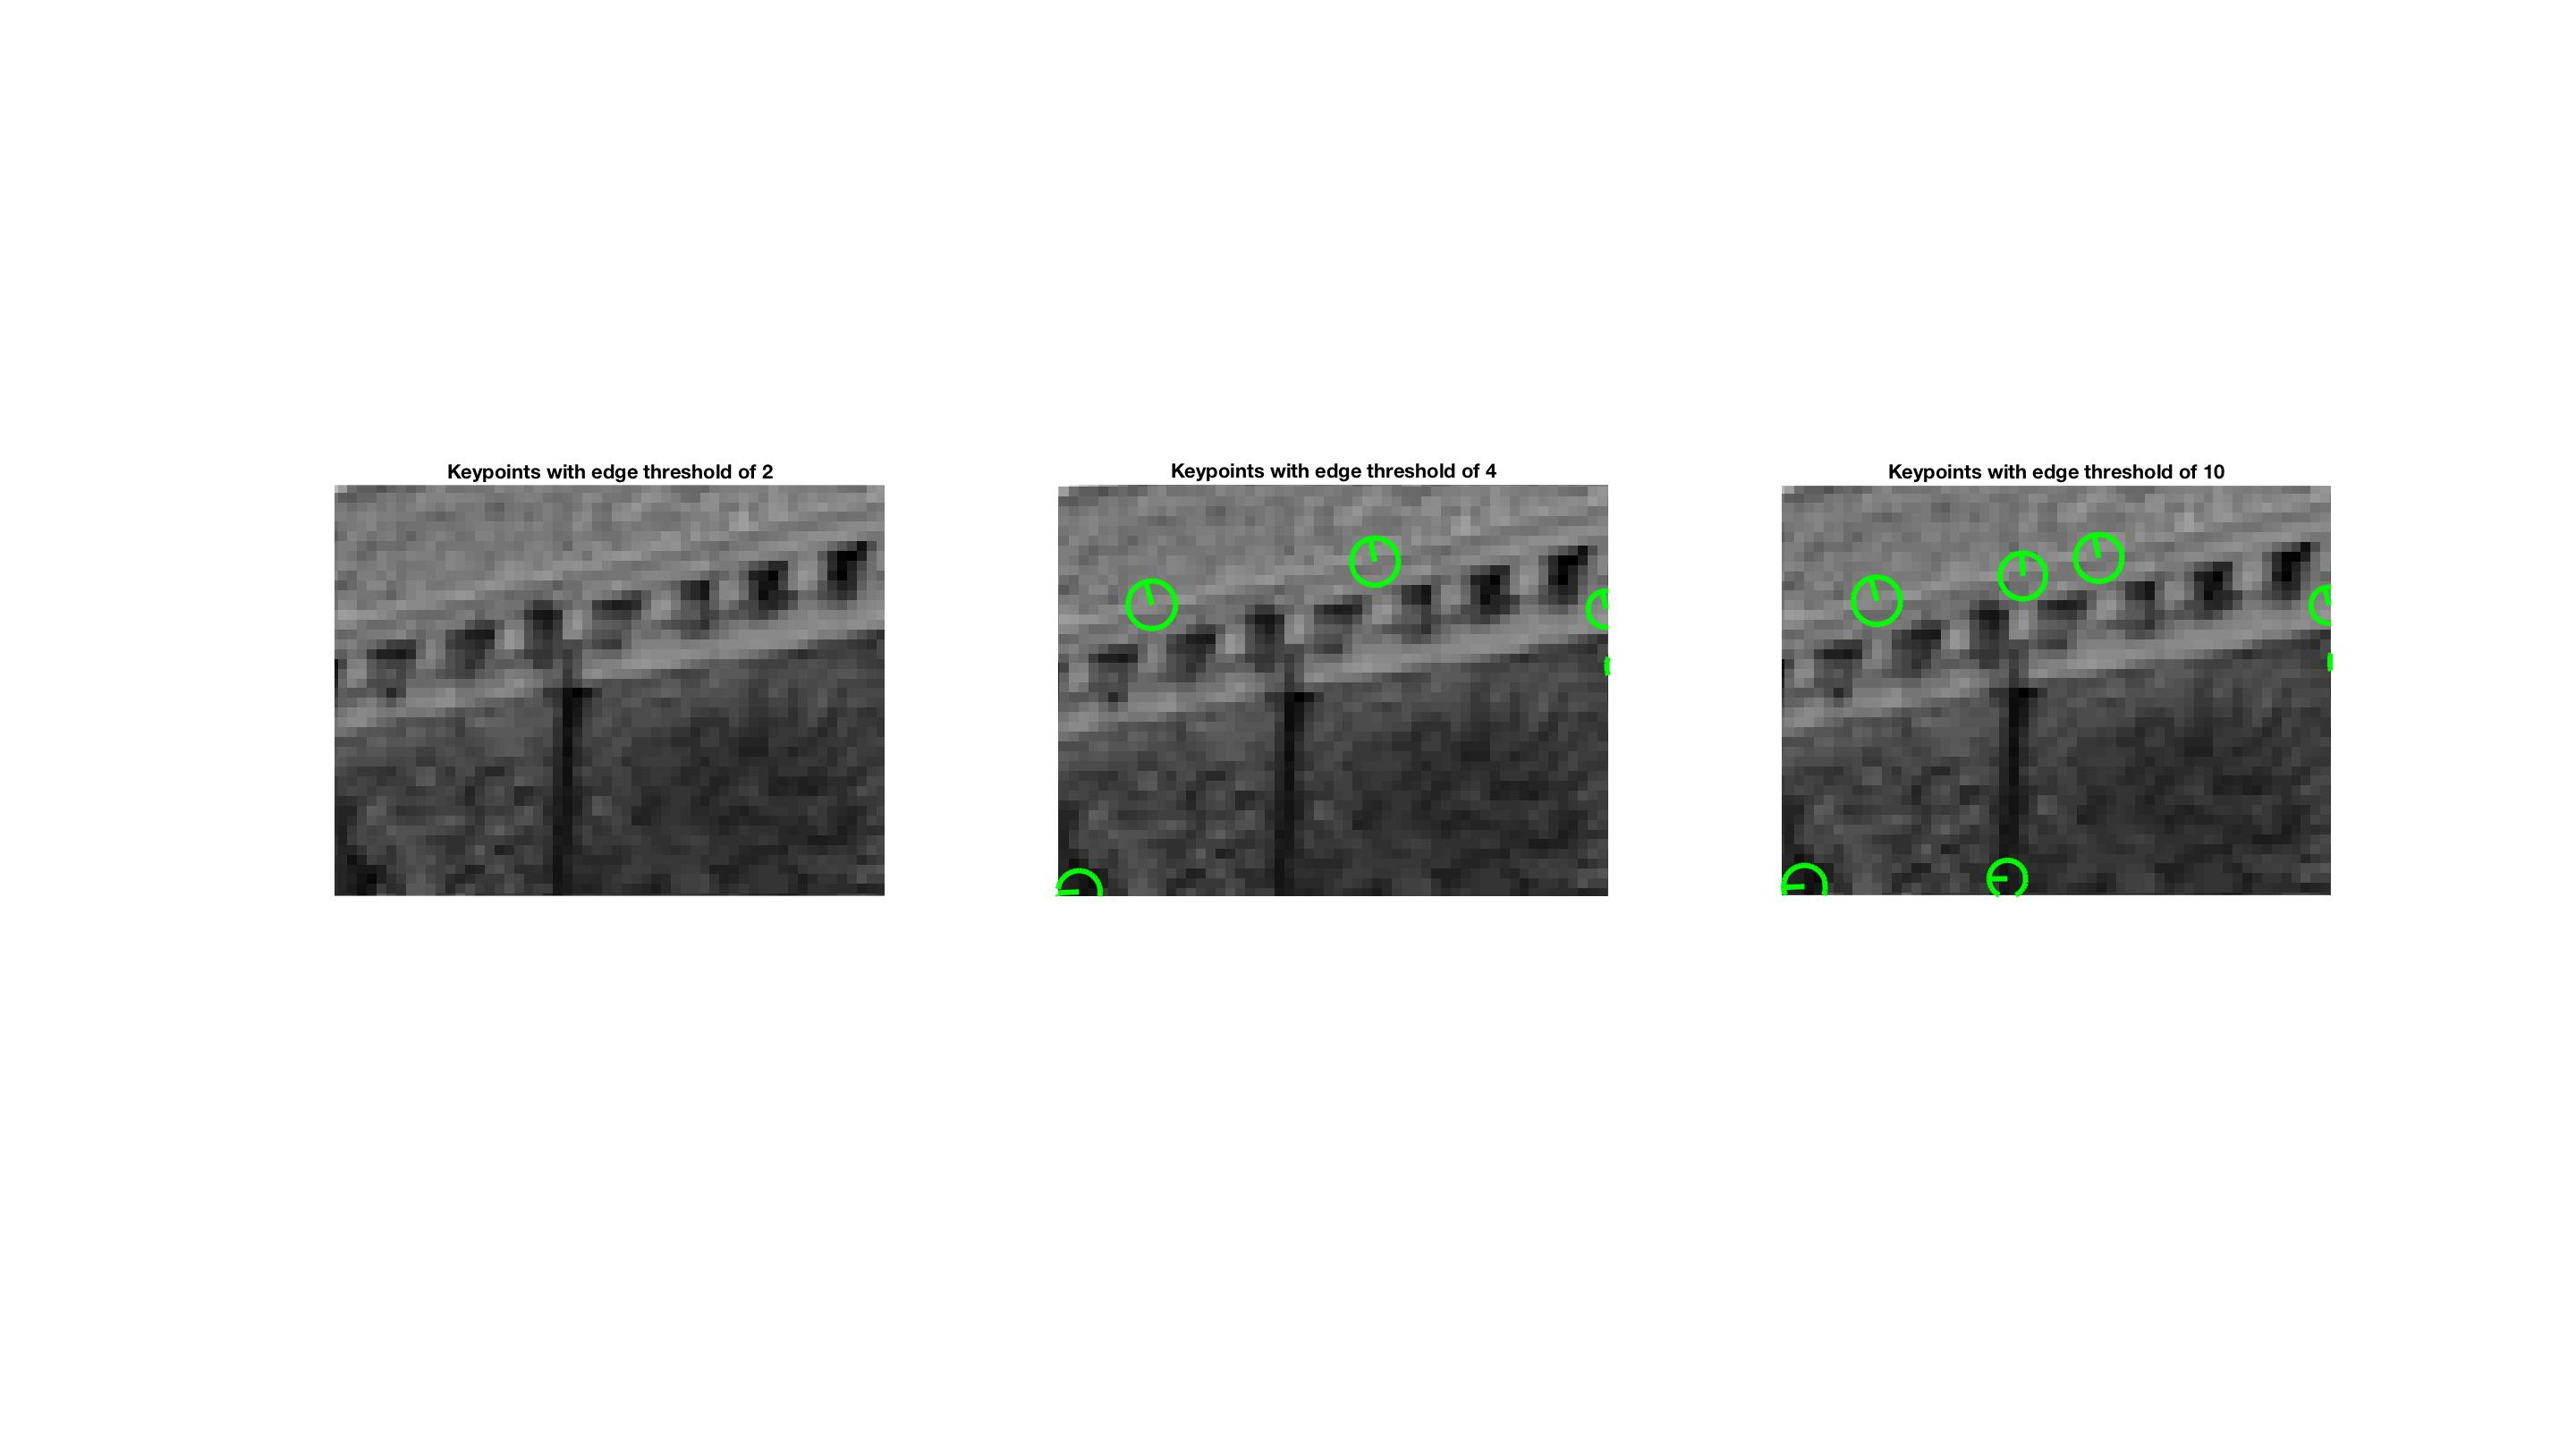
\includegraphics[width=\textwidth]{img/inc_edge_thresh}
  \caption{Effects of decreasing the edge threshold}
  \label{fig:inc_edge_thresh}
\end{figure}

As we can see in figure \ref{fig:inc_edge_thresh}, low values of the edge threshold effectively remove keypoints that lie along edges. The edge threshold r is the ratio between the largest magnitude eigenvalue $ \lambda_{max} $ and the smaller one $ \lambda_{min} $ with $ \lambda_{max} = r \lambda_{min} $. A small r means that both eigenvalues are relatively close to each other, which indicates a high curvature. With decreasing $ r $ we remove more and more keypoints on edges. This effect can be observed in figure \ref{fig:n_peak_thresh}: While there are no keypoints with a ratio $ r $ that is exactly 1, for increasing the edge threshold we allow more and more keypoints that lie on increasingly obvious edges. This fits to our expected behavior based on the way the threshold is defined. 

\begin{figure}[!hbt]
  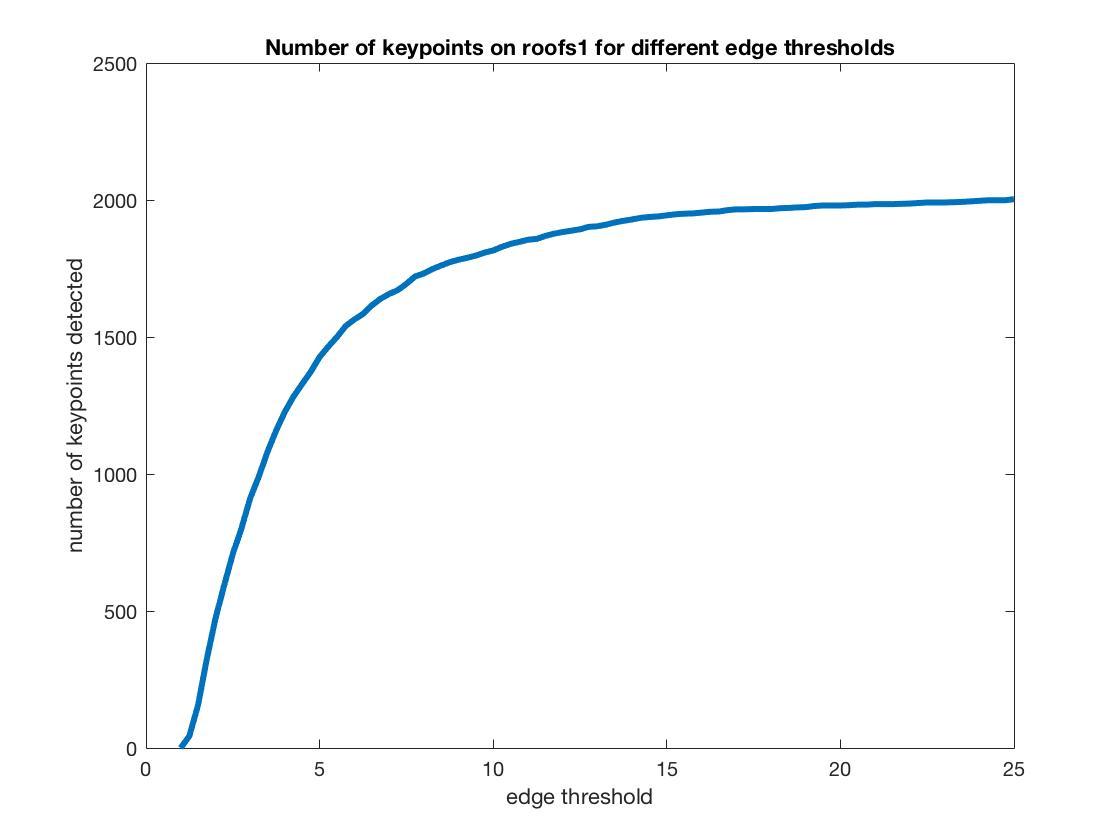
\includegraphics[width=\textwidth]{img/n_edge_thresh}
  \caption{Relationship between edge threshold and number of detected keypoints}
  \label{fig:n_peak_thresh}
\end{figure}

